% \documentclass{proc}
% \documentclass[journal, letterpaper]{IEEEtran}
\documentclass[9pt,journal,compsoc]{IEEEtran}
\usepackage{listings}
\usepackage{fancyvrb}
\usepackage{framed}
\usepackage{ragged2e}
\usepackage[listings,skins]{tcolorbox}
\usepackage[skipbelow=\topskip,skipabove=\topskip]{mdframed}
\usepackage{pbox}
\usepackage{graphicx}
\usepackage{url}
\usepackage{hyperref}
\usepackage{caption}
\linespread{1.1}
\usepackage{float}
\setlength{\parskip}{0.4em}
\usepackage{subcaption}

\mdfsetup{roundcorner=0}
% Congyang: Added the geometry module to add the margin of bottom
\usepackage[top=1in, bottom=1.2in, left=0.7in, right=0.7in]{geometry}
% Congyang: Added the indent first module (and delete "\\" of every paragraph) to make it indent every paragraph.
\usepackage{indentfirst}

\begin{document}

\title {\Huge Visualization Interactivity Perception Research \\ on Data Journalism}
% \textbf{}
% \huge

\author{Congyang Wang, Xiaoqun Wang, Yimin Lin \\ Department of Data Science -- Worcester Polytechnic Institute, MA, 01609 \\ Email: \{cwang8, xwang16, ylin6\}@wpi.edu}

\IEEEtitleabstractindextext{%

\begin{figure} [H]
  \centering
%   \captionsetup{width=0.7\textwidth}
  \begin{subfigure}{.3\textwidth}
  \centering
  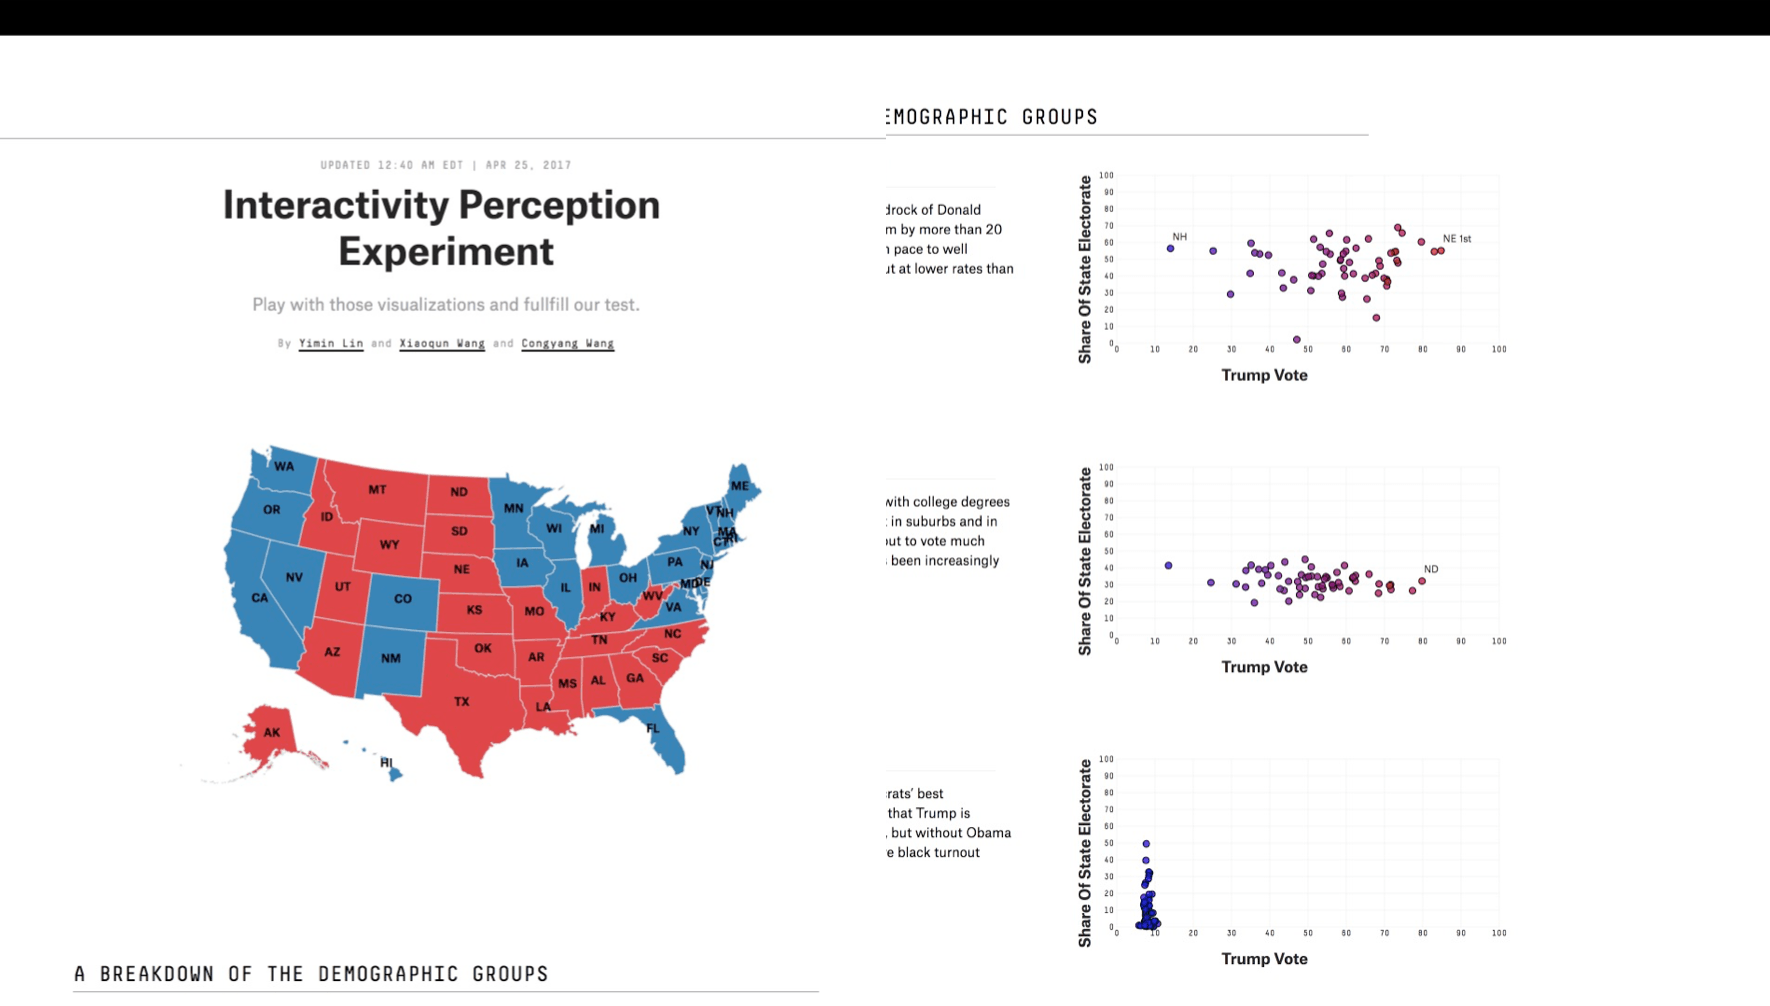
\includegraphics[width=0.84\textwidth]{level0.png}
  \caption{Level 0: No Interactive}
  \label{}
  \end{subfigure}%
  \begin{subfigure}{.3\textwidth}
  \centering
  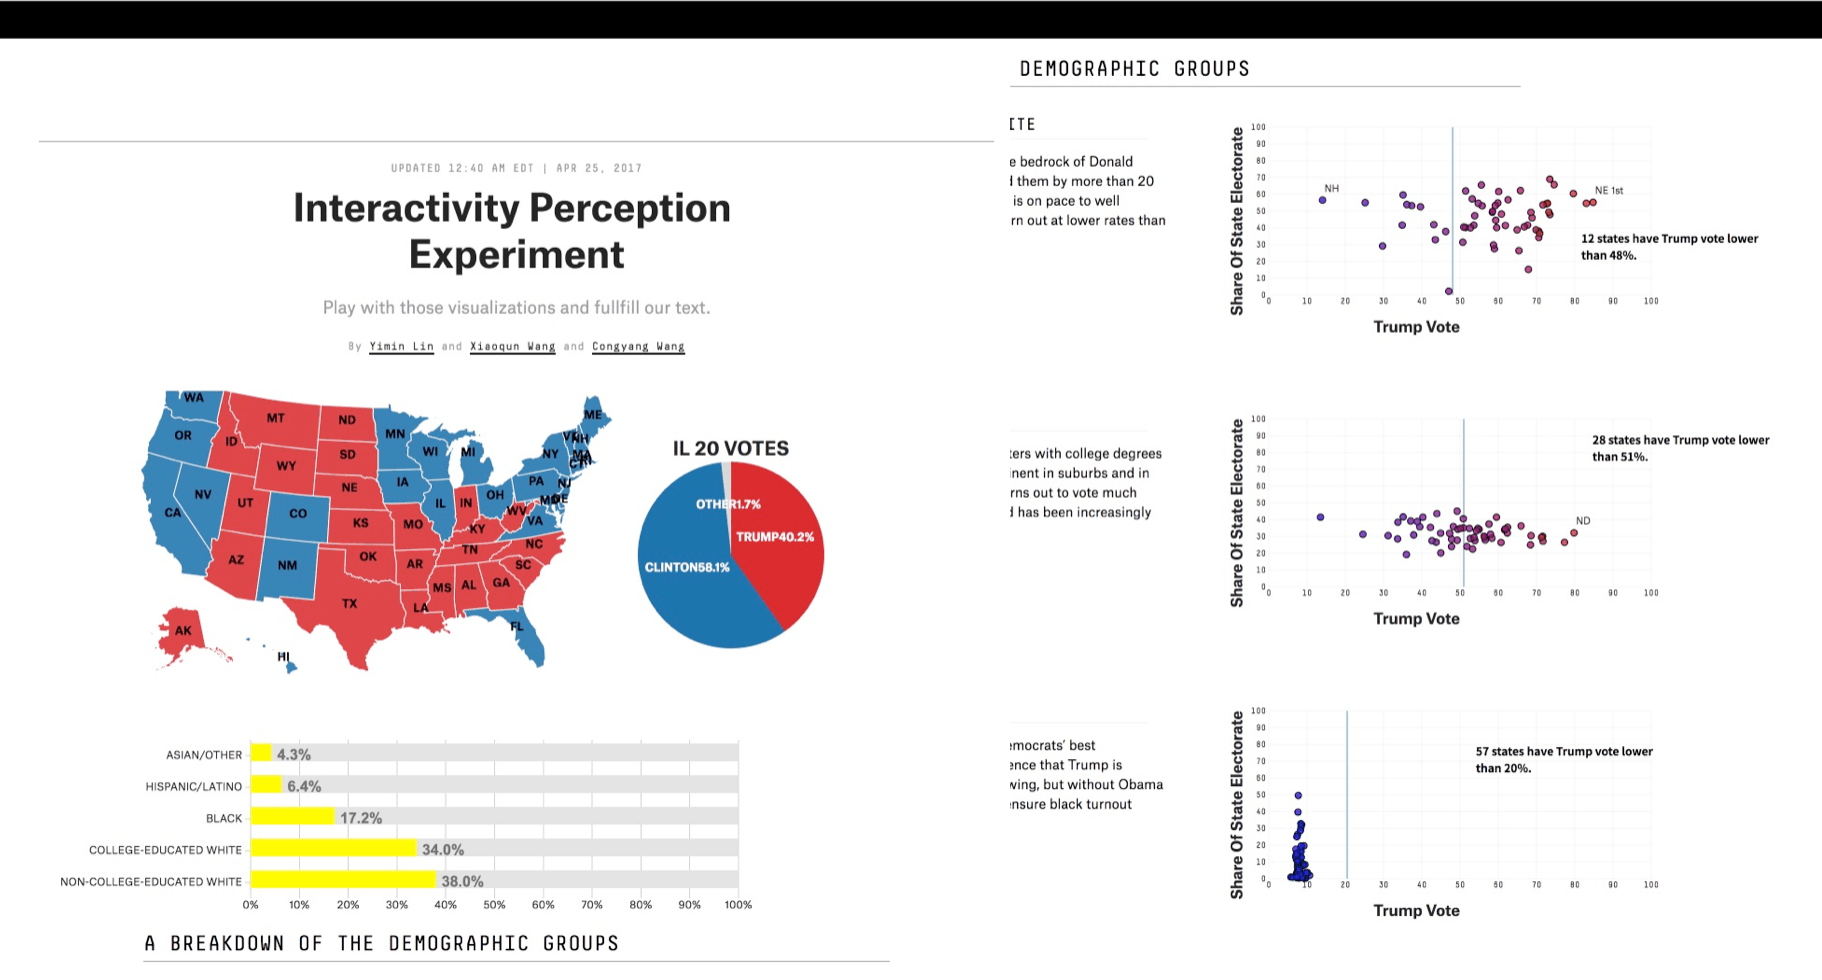
\includegraphics[width=0.89\textwidth]{level1.png}
  \caption{Level 1: Semi-Interactive}
  \label{}
  \end{subfigure}%
  \begin{subfigure}{.3\textwidth}
  \centering
  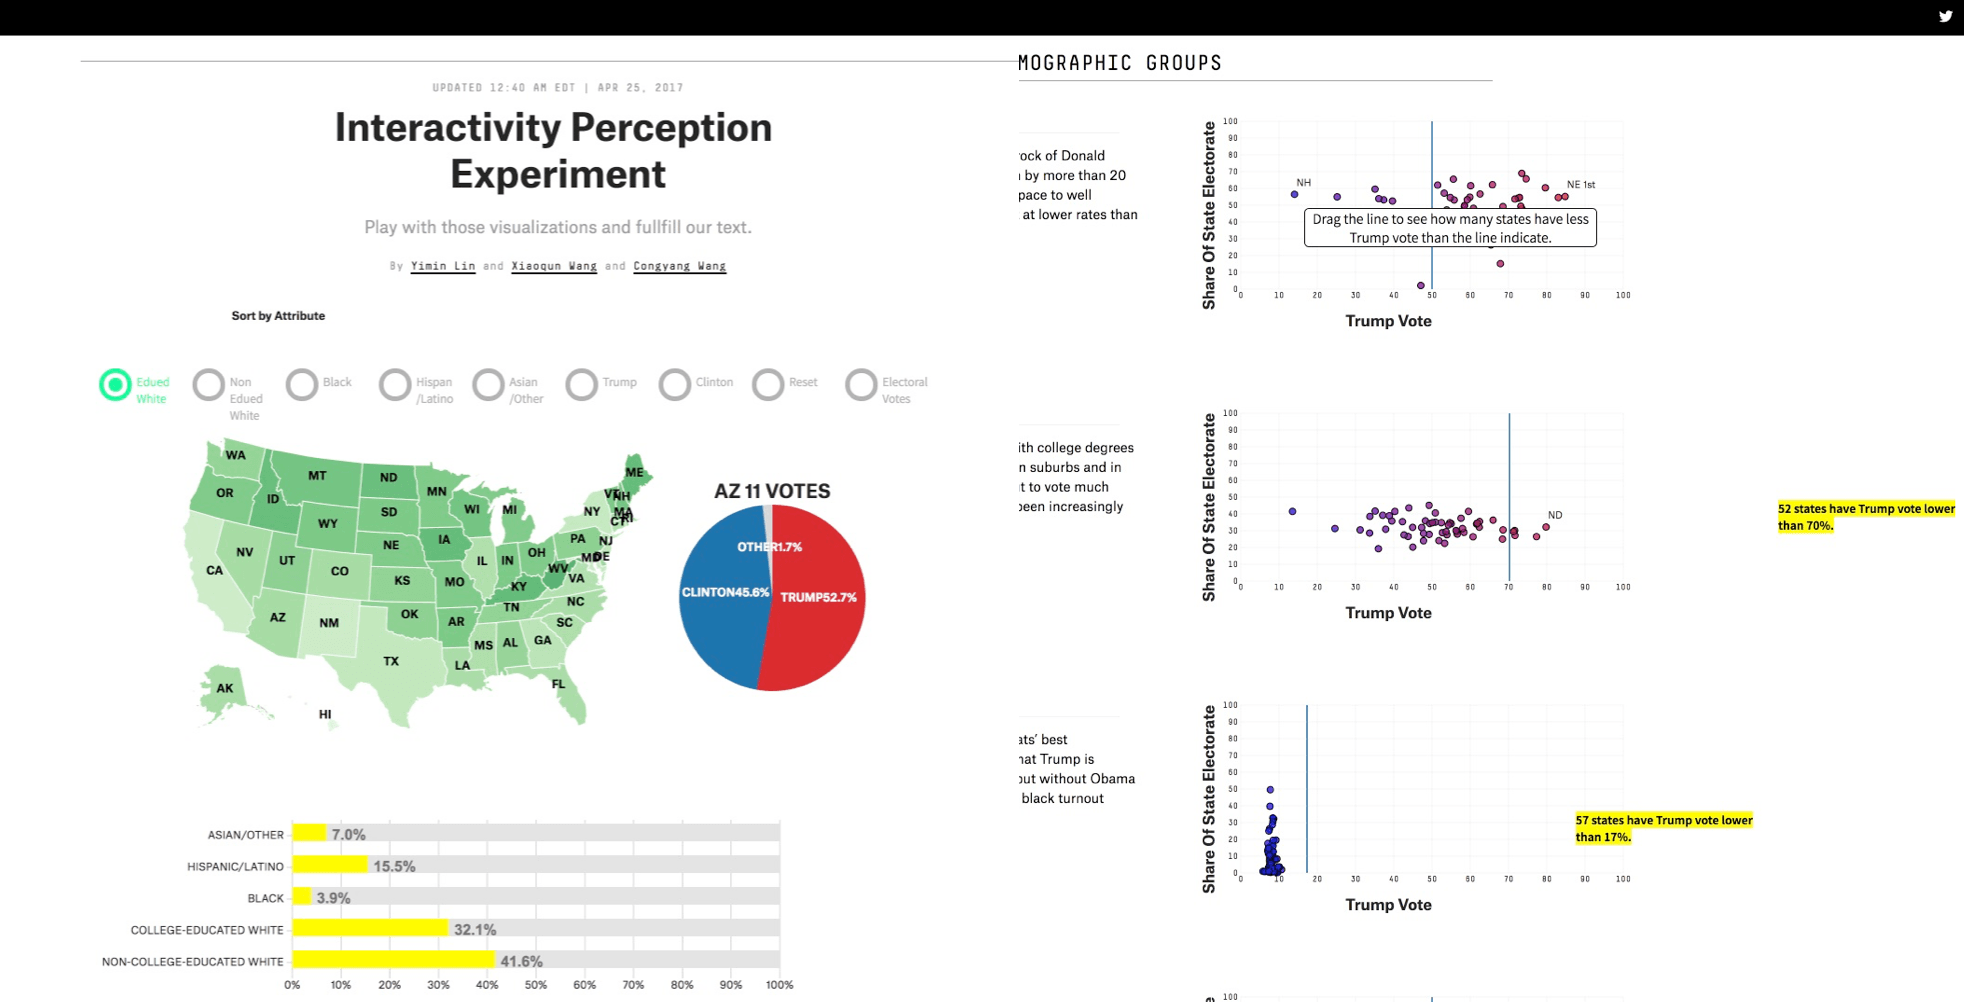
\includegraphics[width=0.93\textwidth]{level2.png}
  \caption{Level 2: Full-Interactive}
  \label{}
  \end{subfigure}
  \label{fig:1}
  \parbox{16cm}{\caption{Here is the application and experiment [13,14,15] with our 3-LEVEL Interactive Comparison method. We applied it to a FiveThirtyEight article about the American Presidential Election with more and more tool-tips, figures, buttons, and tips to upgrade the interactive level.}}

\end{figure}

\begin{abstract}
\justifying
The journalism is growing with a very high speed with the boom of Internet, no matter the traditional media or the emerging social media all join this information revolution in past 20 years; Meanwhile, the data science started to join this revolution in recent years. With the more and more data involved in the journalism, there is new upgrade journalism appears the Data-Driven Journalism. The journalism content revolution starts from the text-only, then, the text with pictures, finally, the text with data visualization. The FiveThirtyEight is a good representative of them. Many articles from FiveThirtyEight suggested from the data, then the editors use all kinds of visualization tools try to show the best interpret of the news to the audiences.    

Unfortunately, there is no evidence shows all kinds of the visualization suit to the explain of data and news, especially for the visualization interactivity, there are many articles in data journalism carried fancy interactivity, but there may only have fewer readers did the interactive with the visualization [1]. 

In this paper, we collected all the visualization interactivity approach, organized and analysis them. Then we designed a multivariate test which use the same article from novel media with different visual interactivity to evaluate the effectiveness of different visual interactivity methods.
\end{abstract}

% Note that keywords are not normally used for peer review papers.
\begin{IEEEkeywords}
Multivariate, Experiment, Visualization, Interactive, Data Journalism, \LaTeX.
\end{IEEEkeywords}}

\maketitle

\section{Introduction}
\large
There is fast growing in the journalism with the current the Internet blooming. Not only the traditional media which may more once focus on the photos in the articles, but also the emerging social media, they all joined this information change, to involve more data-related plots and figures to make the concept and the main idea of the article delivering more clearly and the details looks more attractive.

At the same time, the data science, a latest and hottest thing started to join this revolution in these years; this is owing to the data growing with the significant speed with more and more people connected to the Internet all day. This situation captured by most of the medium, so this is upgraded action happening in recent years: The journalism content changed from the text-only to the text with data visualization. Every time we talked about the data journalism, we can not skip the FiveThirtyEight, which is famous for its abundant data-driven articles.

But, how the interactive and user experience revolution affect the audience behavior of the online news website? We have no answer yet, so we made a 3-LEVEL Interactive Comparison method, which can collect the audience behavior data to analysis the different level interactive influence through the multivariate test on the same one data-driven article. In this method, at first, we deliver the no interactive news page, then we deliver news with part of interaction like tooltips and mouse hover. Finally, we deliver the news with tips about how to use the interaction and the bi-direction interaction (direction-1: Overview to Detail, direction-2: Detail to Overview). To collect the results of audience pattern cognition about the main idea and some details of this article, we also build a back-end system with a questionnaire to collect the time spend of the audience.

Through this practical experiment, we dedicate to explore the relationship between user perception and interactive, four hypotheses are proposed in our study, which is listed in Section 3.

 To verify this hypothesis, we designed a 3-level comparison interactive method which with the three levels of the interactive and visualization on the same article, then collect the users stay time with the content understanding questionnaire through the back-end information collect system. 

To evaluate our method and hypothesis, we used a real-world article from FiveThirtyEight.com and reproduced it with three versions then put it online. This article contains the information about 2016 US presidential election, include the voting rate for Trump among different states and different race.

The rest of this paper is organized as follows. We begin in Section 2 and discuss related work. We then present and discuss our novel method and the experiment details in Section 3. In Section 4, we evaluate the experiment results then visualize and analysis how the method works out. Finally, we discuss the merits and shortcomings of this approach and experiment, suggest directions for future work, and draw our conclusions.

\section{Related Work}
\large
As a lot of researches shown, the basic idea of the visual representation is to efficiently interpret what is behind of the visualization, make it as easy as possible to understand. In this fasting world, there are already many availability visualizations and interactive techniques we can use, meanwhile it always made us confuse to know what and when should be an appropriate technique to use to deliver a possible understanding [5]. There is a large body of work that studies techniques for visualization [1,3,4,8]. At the same time, there is already have a good begging of the study of the interaction in the visualization [2,6,7,12]. From these papers, we captured the current research progress of the interactive visualization application.

Khan [5] introduced a guide for the young researchers what the different available visualization techniques are and how to choose one with specific convey the different level of understanding. In the paper, the author collected all visualization techniques and their brief introduction. From the paper, we knew more visualization methods and had a concept that the interactive and animated visualization is more beneficial to convey the conclusion of the huge data set which is harder to understand under traditional approaches. But it didn't show an experiment or a case study to evaluate this theory which we conducted on the data journalism.

To study the user perception of interactivity, Cheng [17,20] proposed some different levels of interactivity and measured users responses on these levels and divided the participants to several groups, each group just take one level of experiments. To measure the experiments, different kinds variables are considered in their test, including liking, time spend to answer questions, related perception questions. Based on the perception result, some researchers [16,17] also explored whether a high interactivity would bring a positive effect on web owners. Robert E[18] explored how users perceive the interaction and proposed six leverage points to help design interactivity. Huei [19] explored how interaction can boost the learning efficiency in online course. Bum [20] explored how interaction can help learning visualization.
  
These articles, methods, and experiments gave us a lot of knowledge of the visualization and interactive industry [5,9,10],  more focus on a general performance research, not a particular area, like the website, mobile website. So it may give us thinking, how about the interactive effectiveness on the fast growing data journalism. The data journalism has become an integral part of several news organizations online strategies. At the same time, the new organizations see data journalism as a part of the transition moving from a news-and-information site towards becoming more interactive a combo of news and information platforms [11]. Based on this ground truth, we can have an expectation of the future of data journalism and the related studies.   

\section{Experiment}
\large
\begin{table}
	\centering
		\begin{tabular}{|c|c|c|c|}
		\hline
     	&Level 0&Level 1&Level 2\\
     	\hline
            		&Static diagram&Drag & Level 2 plus\\ 
        Interactive& with tool tips&Multiple Charts& instruction\\
					&             &   			&Sort Buttons\\
     	\hline
        \end{tabular}
     \caption{Three level of Interactive}
\end{table}
\subsection{Hypotheses}
Based on the related work, we decide to divide the interactivity perception experiment into three levels. The hypothesis we put forward are listed as follows.\\
\textbf{Hypothesis 1.} Users are easier to perceive the information with higher interaction.\\
\textbf{Hypothesis 2.} Users are more willing to engage in the story with higher interaction.\\
\textbf{Hypothesis 3.} Higher level of interactive visualization can improve user's perception for data journalism.\\
\textbf{Hypothesis 4.} Higher level of interactive visualization can reduce the misleading by article.\\

\subsection{Interaction Levels Design}
In this experiment, we design three levels of interactive visualization as indicated in Table 1. To control the noise, all of the three levels of interactive visualization are embedded in a news website.\\
\textbf{Level 0:} Designed with zero interaction. The website contains the original article, and static U.S. map, scatter plot, with tool tips that demonstrate the given data. \\
\textbf{Level 1:} Designed with some interaction such as drag, mouse over effect, hover multiple charts. \\
\textbf{Level 2:} Finally, for this design, the bi-directional visual interaction pattern is used. Buttons to sort attributes are also introduced. These interactions are implemented based on U.S. map and scatter plot.

\begin{figure*} 
  \centering
%   \captionsetup{width=0.7\textwidth}
  \begin{subfigure}{.33\textwidth}
  \centering
  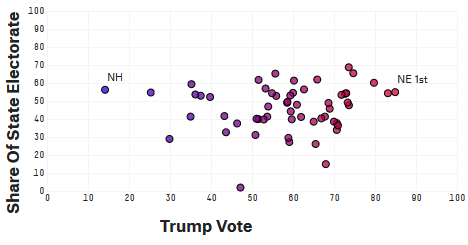
\includegraphics[width=0.84\textwidth]{ScatterLv1.png}
  \caption{Level 0: No Interactive}
  \label{}
  \end{subfigure}%
  \begin{subfigure}{.33\textwidth}
  \centering
  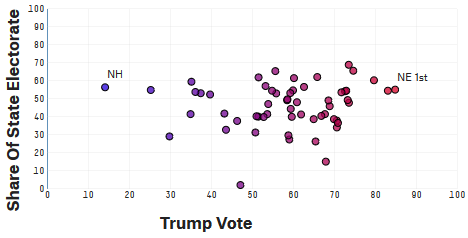
\includegraphics[width=0.89\textwidth]{ScatterLv2.png}
  \caption{Level 1: Semi-Interactive}
  \label{}
  \end{subfigure}%
  \begin{subfigure}{.33\textwidth}
  \centering
  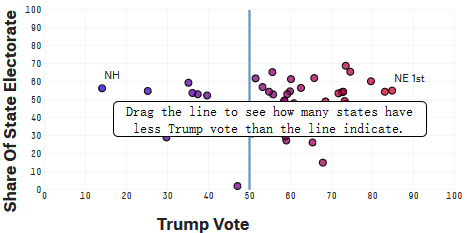
\includegraphics[width=0.93\textwidth]{ScatterLv3.png}
  \caption{Level 2: Full-Interactive}
  \label{}
  \end{subfigure}
  \parbox{17cm}{\caption{The 3-Level interactive scatter plot. (a) shows non-interactive static scatter plot. (b) implements the drag interactive for the static plot without instruction. (c) implements the drag interactive for the static plot with instruction.}}
\label{fig:1}
\end{figure*}

\textbf{U.S. Map:} For U.S. Map, we want to explore whether users are easier to find patterns through the help of interactivity, whether they are more willing to play with the interactivity and whether users are more likely to perceive date when multiple views applied.In this part, four questions were designed for this part. For level 0, the map is filled with two colors; a tooltip was introduced to provide detailed information for each state. For level 1, the map is equipped with two other charts; users can directly find the information with the help of multiple charts rather than simple scan through the tool tip. For level 2, buttons with sort functions are introduced, which aims to help users to recognize the pattern among states.

\textbf{Scatter Plot:} For scatter plot part; we want to explore whether the higher level of interactive can improve user's perception, and reduce the potential misleading by the article. There are two questions in a questionnaire designed for this investigation. For the level 0, as shown in Fig. 2(a), the static scatter plot contains the necessary information is displayed for users without any interactive visualization and instruction. Users were expected to find out the correct answer by the naked eye. For level 1, as shown in Fig. 2(b), we add the drag interactive on the left side of this scatter plot. The user can draw the line on the plot, the information about how many states has lower Trump vote will demonstrate in the tool tip. The purpose of this interaction is to help the user find out the accurate number of states with lower Trump vote than the line indicate, users have to figure out the usage and the information displayed on this interactive without instruction.  For level 2, as shown in Fig. 2(c), we add the instruction on top of the level 1 design. 

\subsection{Test Design}
To explore the hypothesis, we designed a test for users. Users can click the button to start the test. Six questions were designed for this test. Four questions for U.S Map and two questions for Scatter Plot. We also record the time spend on each question.\\
\textbf{Q1: }What's the vote rate for Trump in KS?\\
This question is designed to explore whether users would find the answer faster if we introduced multiple charts\\
\textbf{Q2: }Among CA, NV, UT, AZ, in which of the following state do Non-Colleged White has the highest vote proportion?\\
This question is designed to explore whether the multiple charts would help users to compare the information faster.\\
\textbf{Q3: } 3. Which of the following statement is TRUE?\\
- In Southeastern Region, BLACK has higher vote proportion than other regions.\\
- In general, Colleged White has higher vote proportion than other group\\
- In FL, CLINTON got lowest vote rate than ssibling states.\\
- It's too hard to find. I choose to skip.\\
This question is designed to explore whether users will use the sort button to find the pattern.\\
\textbf{Q4: }In CA, FL,TX, which of the state has the HIGHest HISPANIC/LATINO vote proportion?\\
This question is designed to explore the effect of multiple charts and sort button.\\
\textbf{Q5: }For college-educated white group, how many number of states with Trump vote rate smaller than 50 percent?\\
This question is designed to test whether the level of interaction can improve the ability of information mining. The correct rate of answering and the time spend were collected for further evaluation. \\
\textbf{Q6: }For Latino group, compare to Romney at 2012, does Trump receive lower vote?\\
This question is designed to test whether a higher level of interactive visualization can reduce the misleading by the article. For the demon graphic part in the article, we deliberately modify the original description part of Latino group. The context of the description: "Latino voters are about 11 percent of the eligible electorate in 2016, up one percentage point from four years ago. Romney received just average 15 percent of their votes in 2012, and Trump is in danger of faring even worse. ",  which indicate Trump is "in danger" to receive lower rate than Romney's 15 percent vote. The actual 2016 Trump vote among Latino group is 28 percent, the user can find this information by draw the line on the scatter plot. The misleading text will lead the user to the wrong answer if they choose to take ambiguous word rather than the real information conveyed through the interaction. 

\begin{figure*} 
  \centering
%   \captionsetup{width=0.7\textwidth}
  \begin{subfigure}{.33\textwidth}
  \centering
  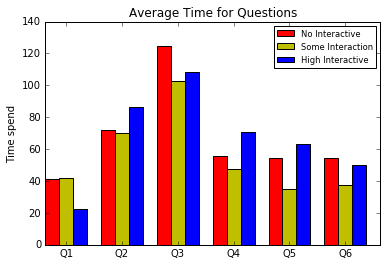
\includegraphics[width=0.84\textwidth]{AverageTimeforMap.PNG}
  \caption{Average Time Spend}
  \label{}
  \end{subfigure}%
  \begin{subfigure}{.33\textwidth}
  \centering
  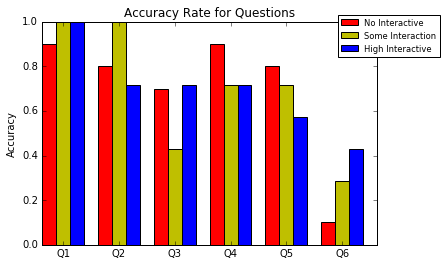
\includegraphics[width=0.89\textwidth]{AccuracyRateforMap.PNG}
  \caption{Accuracy Rate}
  \label{}
  \end{subfigure}%
  \begin{subfigure}{.33\textwidth}
  \centering
  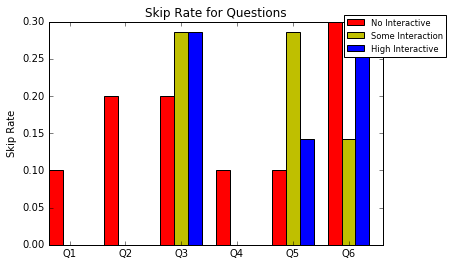
\includegraphics[width=0.93\textwidth]{SkipRateforMap.PNG}
  \caption{Skip Rate}
  \label{}
  \end{subfigure}
  \parbox{17cm}{\caption{Time Spend, Accuracy Rate and Skip Rate for three levels. (a) shows the average time spend on each question. (b) shows the average accuracy rate for each question. (c) shows the skip rate for each question.}}
\label{fig:1}
\end{figure*}

\subsection{Participants}
26 of our classmates are invited to take this experiment. To exclude another factor of influence, we divided users into three groups. Each of the group takes one interactivity level only once. They received the link to the website and took the experiment remotely. After finished the experiment, their response will be sent to our email automatically. We got ten responses for Level 0, eight responses for Level 1 and eight responses for Level 2.

\section{Evaluation}
\large
\subsection{Data Preprocessing}
The Fig.3 shows the box plot of time spends for each question. We can see that there are some extreme low values at the button. When we scan through the corresponding answers, we found that the accuracy and skip rate are also lower than expect. Based on such fact, we assuming that people spend 5 seconds less on each question is not taking the test seriously. In the following evaluation, we exclude the responses that spend less than 5 seconds on average for each question to make our analysis more convincing.
\begin{figure} [H]
  \centering
  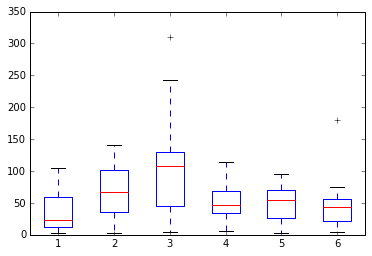
\includegraphics[width=0.32\textwidth]{TimeSpendBox.PNG}
  \caption{Time Spend for Each Question}
  \label{fig:6}
\end{figure}
\subsection{Time Spend Evaluation}
Fig.4(a) shows the average time spend for three levels in each question. From the bar chart we can see that in general, users tend to spend less on Level 1 than Level 0. However, when it comes to the high interactivity(Level2), the results shows that the users might spend more time on answering questions.

\begin{figure} [H]
  \centering
  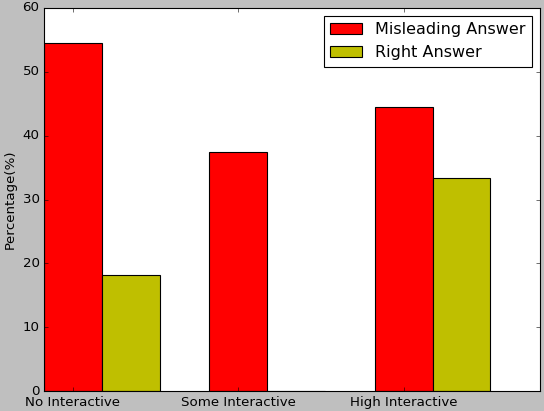
\includegraphics[width=0.32\textwidth]{MisleadingQ6.png}
  \caption{The comparison between the "Misleading Answer" and "Right Answer".}
\end{figure}

\subsection{Accuracy and Skip Rate Evaluation}
\textbf{Accuracy Rate.} Fig.4(b) shows the average accuracy rate for three levels in each question. For Question 1-4(Map Visualizations), the average accuracy rate of each level shows somewhat random, but combined with the skip rate, we can gain some insight from them. For Question 5-6 (Scatter Plot Visualization), the average accuracy rate is expected to proportionate to the level of interactive due to the design of issue. 

\textbf{Skip Rate.} Fig.4(c) shows the average skip rate for three levels in each question. For Question 1-4(Map Visualizations), the level 0 shows a significant high skip rate than other two levels of interactivity. \\



\section{Discussion}
\large
\subsection{Test Result Findings}
This part will discuss the test result in details and conclude the insights from the test result.

For Question 1-4, time spends for Level 1 is less than Level 0, while time spends for Level 3 is more than the other two. So we can conclude that Some interactivity could help users to recognize the data faster. However, if the interactivity is too complex, users might have trouble to use the interaction. Therefore, designers must measure the complexity of their interactivity. The accuracy rate is random, so we can conclude that unsuitable designed interactivity can cause a misleading effect. However, since the Level 0 shows a significant higher skip rate in Question 1-4, we can conclude that the rich interactivity would make users engage more in the test. The low skip rate of Level 1 and Level 2 indicates that a rich interactivity would make users more willing to participate in the test and feel more confident on the test.
For question 5, surprisingly, the higher interactive level doesn't help users to get higher correctness. This may because the points in the scatter plot are clearly separated,  users could make a judgment by naked eyes. So the information obtained from the interactive doesn't help in this case. For question 6, the improvement of correctness from interactive is prominent. The higher interactive can help users to find the approximate average Trump vote, and decrease the influence of context misleading. On the other hand, the relatively high skip rate may result from the less passionate of reading. In order to answer this question, users have to read the context throughtly, which may decrease users willing in answering. In this problem, if users are misleading by the context, they will tend to choose "Yes" over the correct answer "No." To further demonstrate the reduce of misleading, we compare the rate of "Misleading Answer" and "Right Answer" as shown in Fig. 5.

\subsection{Limitations and Future Research}

We took a step out to evaluate if the different level of interactive can affect the audience of the newspapers online in data journalism. For the experiment itself, we used five kinds of the common interactive methods, as the front-end technology fast changing, the future research should consider not only the classic methods but the latest visualization technology. Meanwhile, with the time limitation, we can not find a more random sample to join this experiment, it should be improved in the future work.

In the next stage, we decided to make a crowd-source experiment and collect more different kinds of data-driven news like entertainment and sport to balance the bias of the different audience reading preference, to make the result more convincing.

In the time spending part, the significant higher time spending for high interaction, which might cause by the complexity. In the next stage, we can add a new group of participants that was introduced how to use these visualizations first. Measure the time spending, and accuracy/skip rate of this group might bring more insights. What's more, a more careful design of interaction need to be considered since the accuracy rate of Level 2, and Level 1 didn't outperform Level 1, which might be caused by lacking the learning stage for interaction.

\section{Conclusion}
\large
The visualization is developing over twenty years, the interactive on the visualization also being studied for decade years. But the data journalism booming is just started. Finding out what are the chemical reactions and the catalyst inside the interactive visualization in the data journalism is a hot study area now.

In this paper, we did a 3-Level experiment to measure the influence of the different degree of data interactive to the data news in the data journalism.  Level 0 for the original article, Level 1 for the visualization with light Interactive, Level 2 for the bi-directional visual interaction. In the experiment, the 3-Level visualization all bounded on the same article. Then we evaluated the visitor stay time data to analysis the effect of interactive of the different level.

The result showed that users are more likely to engage in the interactivity. Users can perceive the information faster than no interactivity while a complex interactivity might make users confused and cause a misleading result.


\begin{thebibliography}{99}
% \large 
\bibitem{c1} Gray, Jonathan, Liliana Bounegru, and Lucy Chambers. \textit{The Data Journalism Handbook} Oreilly \& Associates, 2012.
\bibitem{c2} Howard J.Seltman, \textit{Experimental Design and Analysis}, Carnegie Mellon University , Department of Statistics
\bibitem{c3} Anthony C. Robinson*, and Chris Weaver, \textit{Re-Visualization: Interactive Visualization of the Process of Visual Analysis}, GeoVISTA Center, Department of Geography, The Pennsylvania State University. 
\bibitem{c4} Wibke Weber, Hannes Rall, \textit{Data Visualization in Online Journalism and Its Implications for the Production Process}, Information Visualisation (IV), 2012 16th International Conference.

% Congyang Citation Begin--------
\bibitem{c5} M. Khan and S. S. Khan, “Data and information visualization methods, and interactive mechanisms: A survey,” International Journal of Computer Applications, 2011.
\bibitem{c6} J. Hullman and N. Diakopoulos, “Visualization Rhetoric: Framing Effects in Narrative Visualization,” IEEE Transactions on Visualization and Computer Graphics, vol. 17, no. 12, pp. 2231–2240, 2011.
\bibitem{c7} P. Godfrey, J. Gryz, and P. Lasek, “Interactive Visualization of Large Data Sets,” IEEE Transactions on Knowledge and Data Engineering, vol. 28, no. 8, pp. 2142–2157, 2016.
\bibitem{c8} S. Steensen, “Conversing the audience: A methodological exploration of how conversation analysis can contribute to the analysis of interactive journalism,” New Media \& Society, vol. 16, no. 8, pp. 1197–1213, Sep. 2013.
\bibitem{c9} B. L. Massey and M. R. Levy, “`Interactive' Online Journalism at English-Language Web Newspapers in Asia,” Gazette (Leiden, Netherlands), vol. 61, no. 6, pp. 523–538, Sep. 2016.
\bibitem{c10} P. Bradshaw, L. Zion, and D. Craig, “What is data journalism,” Ethics for digital journalists, 2015.
\bibitem{c11} T. Aitamurto, E. Sirkkunen, and P. Lehtonen, “Trends In Data Journalism ,” Espoo: VTT, 2011.
\bibitem{c12} N. Kayser-Bril, A. Valeeva, and I. Radchenko, “Transformation of Communication Processes: Data Journalism,” arXiv.org, vol. cs.CY. 06-May-2016. 
% Congyang Citation end--------

\bibitem{c13} Web Interactivity Perception Experiment on Real articles L0: https://yiminlin1994.github.io/gradfinal/index1.html
\bibitem{c14} Web Interactivity Perception Experiment on Real articles L1: https://yiminlin1994.github.io/gradfinal/index2.html
\bibitem{c15} Web Interactivity Perception Experiment on Real articles L2: https://yiminlin1994.github.io/gradfinal/index3.html 
\bibitem{c16} J. E. Guillory and S. S. Sundar, “How Does Web Site Interactivity Affect Our Perceptions of an Organization?,” Journal of Public Relations Research, vol. 26, no. 1, pp. 44–61, Jan. 2014.
\bibitem{c17} C. Yi, Z. J. Jiang, and I. Benbasat, “Enticing and Engaging Consumers via Online Product Presentations: The Effects of Restricted Interaction Design,” Journal of Management Information Systems, vol. 31, no. 4, pp. 213–242, Apr. 2015.
\bibitem{c18} R. E. Patterson, L. M. Blaha, G. G. Grinstein, K. K. Liggett, D. E. Kaveney, K. C. Sheldon, P. R. Havig, and J. A. Moore, “A human cognition framework for information visualization,” Computers \& Graphics, vol. 42, pp. 42–58, Aug. 2014.
\bibitem{c19} H.-C. Wei, H. Peng, and C. Chou, “Can more interactivity improve learning achievement in an online course? Effects of college students' perception and actual use of a course-management system on their learning achievement,” Computers \& Education, vol. 83, pp. 10–21, Apr. 2015.
\bibitem{c20} B. C. Kwon and B. Lee, “A Comparative Evaluation on Online Learning Approaches using Parallel Coordinate Visualization,” presented at the the 2016 CHI Conference, New York, New York, USA, 2016, pp. 993–997.


\end{thebibliography}
% \begin{enumerate}
% \end{enumerate}
\end{document}